\chapter{Future Work} \label{cha:future}

In this chapter, we will discuss improvements that can be made to this
implementation, and improvements that similar architecture should
consider.

\section{Testing}

There should be tests made to ensure that a module behaves the same, if written
in Rust or JavaScript. This can be an issue, because the way a module interacts
with the \gls*{ide} is through a core, which is implemented separately for the
different module systems. Test modules should be made, ensuring that the end
state of the \gls*{ide} is the same, when the module does the same action. But
this would require the modules being semantically the same for the different
test cases. In any case, difficult to ensure all edge cases have been covered.

\subsection{End-To-End testing}

We cannot guarantee that all the utility methods in the JavaScript and Rust
libraries work as expected. A proper test scenario that covers a wide array of
functionalities offered by the different libraries should be implemented. An
example scenario, is one where two modules, one in the Rust ecosystem, the other
in the JavaScript ecosystem, sending back and forth different values, and
modifying them, using their own implemented methods.

\begin{enumerate}
  \item Both modules receive an event with some argument
  \item Both modules respond with an event, with some complicated argument
\end{enumerate}

We can then assert if the manipulation is like expected.

\section{Language agnosticism improvements}

Steps should be made to mitigate the shortfall of this solution, with regard to
language agnosticism. The differences in installation for \gls*{rsms} and
\gls*{jsms} are mainly due to how trivial it is to install JavaScript modules,
compared to Rust modules. \gls*{jsms} should enforce a similar system of module
building as \gls*{rsms}, not only to ensure less semantic differences, but also
to ensure safety, as restricting the \gls*{jsms} is good.

\section{Attribute and instructions}

Can't remove or change eventListeners currently. This is because to remove an
EventListener, the exact same function passed to the \textit{addEventListener}
must be used, which means a reference to this function needs to be stored, but
having two or more of the same type? It can get confusing for a module developer
of what should actually happen.

\section{Keypresses}

A common feature of \gls*{ide}s is being able to have certain keybindings for
different actions. For example, in \gls*{vscode}, one can hit \textit{CTRL}
$+$ \textit{n} to open up a new tab, with a new file. This system is not yet
possible in the \gls*{ide}, but this is due to a lack of a supporting module
family. But, given that this is a common feature in \gls*{ide}s, this should be
a priority.

\section{Inconsistent UI representation}

Difficult to keep the \gls*{ui} representation consistent with the \gls*{dom}.
An example of this, is that the \gls*{ui} representation in the \gls*{ide} does
not store information like the possible \textit{value} an \gls{html} might
have. So for the editor module, there is no efficient way to know what text is
in the editor. Another example, is for the module installer, there is no way for
the module to \textit{query} the \gls*{ui} for information about the form it
presents the user, seeing what values are in the fields. A workaround to this
was used, where depending on what element an \textit{eventListener} was added
to, the sent event would be \textit{sticky}, meaning it would add extra
arguments to the \textit{args} field of the Event, like attribute information,
id, value, etc. But this would not update the \gls*{ui} stored in the
\gls*{ide}, but rather give modules a peek at the current \gls*{ui} state. A
better solution would be to somehow keep track of \textit{all} user interactions
to the \gls*{dom}, and somehow bubble these changes down to the backend, where
the \gls*{ui} representation is managed.

\section{Unify the tooling}

A \gls{cli} tool should be made for users to add compile-time modules.
Currently, a user has to specify what kind of module they are adding, the
language and package manager if it is a JavaScript module. This is trivial to
detect by a program. A user should be able to simply invoke the tool with
either a URL or a path to the module, and then the tool can infer what kind of
module it is, and add it to the configuration file correctly. The same tool
should also include the other tooling, like generating the module dependency
graph.

\section{Modular editor}

The prototype editor module develop for this \gls*{ide} is subpar compared to
existing ones. A new one should be developed, in tandem with a \gls*{ls} client.
This will ensure that this \gls*{ide} can support more languages. This editor
should then utilize existing technology that is already used by other
\gls*{ide}s, like the tree-sitter\footnote{\url{https://github.com/tree-sitter/tree-sitter}}
parsing system, which amongst other things, can help with syntax highlighting.

\subsection{Editor buffers}

One of the reasons the prototype editor module is subpar, is that it uses a
textarea \gls*{html}-element as input and renderer of text content. This should
be replaced by a buffer system, similar to how other \gls*{ide}s do. In the
figure \ref{fig:editorBuffer}, we can see a diagram of a module family which
enable a better, more modular, editor.

\begin{figure}
  \centering
  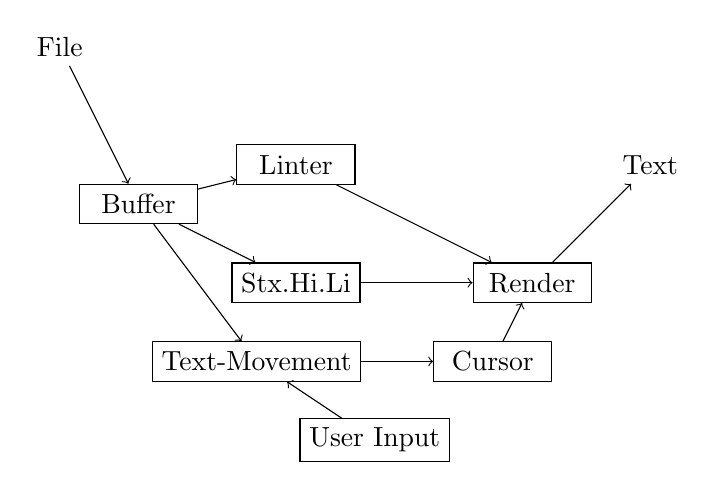
\begin{tikzpicture}
  % Nodes
  \node (file) [] at (-6, 3) {File};
  \node (parser) [rectangle, draw, minimum height=0.5cm, minimum width=1.5cm] at (-5, 1) {Buffer};
  \node (stxhili) [rectangle, draw, minimum height=0.5cm, minimum width=1.5cm] at (-3, 0) {Stx.Hi.Li};
  \node (text-movement) [rectangle, draw, minimum height=0.5cm, minimum width=1.5cm] at (-3.5, -1) {Text-Movement};
  \node (linter) [rectangle, draw, minimum height=0.5cm, minimum width=1.5cm] at (-3, 1.5) {Linter};
  \node (cursor) [rectangle, draw, minimum height=0.5cm, minimum width=1.5cm] at (-0.5, -1) {Cursor};
  \node (user-input) [rectangle, draw, minimum height=0.5cm, minimum width=1.5cm] at (-2, -2) {User Input};
  \node (render) [rectangle, draw, minimum height=0.5cm, minimum width=1.5cm] at (0, 0) {Render};
  \node (text) at (1.5, 1.5) {Text};
  % Arrow
  \draw[->] (file) -- (parser) node[midway, above] {};
  \draw[->] (parser) -- (stxhili) node[midway, above] {};
  \draw[->] (parser) -- (linter) node[midway, above] {};
  \draw[->] (parser) -- (text-movement) node[midway, above] {};
  \draw[<-] (render) -- (stxhili) node[midway, above] {};
  \draw[<-] (render) -- (linter) node[midway, above] {};
  \draw[<-] (cursor) -- (text-movement) node[midway, above] {};
  \draw[<-] (text-movement) -- (user-input) node[midway, above] {};
  \draw[->] (cursor) -- (render) node[midway, above] {};
  \draw[->] (render) -- (text) node[midway, above] {};
\end{tikzpicture}


  \caption{
    Diagram of a module dependency graph for an editor module family. The
    contents of a file are stored in a buffer, which different modules, linter,
    syntax highlighting and text movement, can handle the text in their
    respective format.
  }
  \label{fig:editorBuffer}
\end{figure}

The general idea is for a buffer to contain the contents of a file. The final
step is for some render module to transform the text into some \gls*{html} that
is actually rendered by the \gls*{ide} to the user. The linter and syntax
highlighter modules add colour to keywords, depending on what language the file
is written in, while the linter adds indications to a user if what they have
written is incorrect, if there is a warning or error. Given that files are just
a long string of bytes, some cursor module is needed, to keep track of where the
user is inserting text. This also allows for other modules, like the text
movement module to register user key presses as text movement.


\section{Improvements to the module architecture}

Other popular \gls*{ide}s have a form of module architecture. For instance, in
NetBeans, modules can directly invoke methods of other modules. This is due to
the modules being written in the same language, and can have the same underlying
\gls*{abi}. We circumvented this issue, by having our \gls*{ide} be the
intermediary, but this restrictions means we can only indirectly invoke the
methods of other modules. An improvement to this architecture, would be for
modules to directly interact with each other, and for the \gls*{ide} itself to be
entirely made out of modules, the only thing the \textit{core} of the zero-core
does, is initialized modules. Letting modules be in charge of their own cycles,
when to be invoked, who to invoke, etc.
